%\documentclass[10pt]{letter}
%\usepackage[utf8]{inputenc}

%%%%%%%%%%%%%%%%%%%%%%%%%%%%%%%%%%%%%%%%%%%%%%%%%
% compile with LuaLatex
%%%%%%%%%%%%%%%%%%%%%%%%%%%%%%%%%%%%%%%%%%%%%%%%%%%%%%%
\documentclass[11pt]{report}
\usepackage{epsfig}
\usepackage{amssymb,amsmath,amsfonts}
\usepackage[activeacute,american]{babel}
%\usepackage[utf8]{inputenc}
\usepackage{subfiles}
\usepackage{cite}
\usepackage{csquotes}
\usepackage{esvect}
\usepackage[acronym,nonumberlist]{glossaries}
\renewcommand{\acronymname}{Nomenclature}
\usepackage{multicol}
\usepackage{caption} 
\usepackage{float}
\usepackage[
    math-style=ISO,      % Upper Case Greek is in italics
    bold-style=ISO,      % Bold math is in italics
    partial=upright,     % nabla and partial upright
    nabla=upright,
  ]{unicode-math}
\topmargin 1.2cm 
\textwidth 16.1cm
\textheight 22.5cm
\oddsidemargin 0.7cm
\setcounter{tocdepth}{5}
\addtolength{\voffset}{-2.4cm}
\addtolength{\hoffset}{-0.5cm}
\usepackage{booktabs}
\usepackage{setspace}
%\doublespacing
\onehalfspacing
\usepackage{caption}
 \captionsetup[figure]{labelfont={bf},name={Figura},labelsep=period}


%%%%%%%%%%%%%%%%%%%%%%%%%%%%%%% 
% citas
% \footnotetext{Mott, Robert L. Mecanica de Fluidos 6/e. Pearson educación, 2006.}
% \footnotetext{Pritchard, Philip J. Fox and McDonald’s Introduction to Fluid Mechanics (8th ed.). John Wiley $\&$ Sons. (2011).}
% \footnotetext{Munson, Bruce R., et al. "Fundamentals of Fluid Mechanics, John Wiley $\&$ Sons." Inc., USA (2006).}
%%%%%%%%%%%%%%%%%%%%%%%%%%%%%%% 

%%%%%%%%%%%%%%%%%%%%%%%%%%%%%%%%%
\begin{document}
\centering{ \textbf{\Large{Mec\'anica de fluidos}}}


\vspace{1cm}

\flushleft{ \large \underline{\textbf{Pr\'actica : Flujos externos viscosos}}}

%%%%%%%%%%%%%%%%%%%%%%%%%
\vspace{1cm}

\underline {Problema 1 (P. 9.43 y 9.44 Fox\footnote{footnotes working fine}):}
\vspace{0.2cm}

Suponga capa limite laminar para estimar la fuerza de arrastre en la placa presentada en la figura~\ref{fig:fig1}, la cual se encuentra paralela a un flujo de aire con velocidad de $15$\,ft/s. El \'aire se encuentra  a 70$^\circ$F y $1$\,atm. Adem\'as, estime la fuerza de arrastre si la placa se gira en $180^\circ$, de forma que la base se enfrenta al flujo, en lugar de la punta.

\begin{figure}[H]
\centering\includegraphics[width=0.4\textwidth]{Figures/9_43F.png}
\caption{\label{fig:fig1} }
\end{figure}

%%%%%%%%%%%%%%%%%%%%%%%%%

\underline {Problema 2:}
\vspace{0.2cm}

Calcule el torque en la base del poste presentado en la figura~\ref{fig:fig2}
\begin{figure}[H]
\centering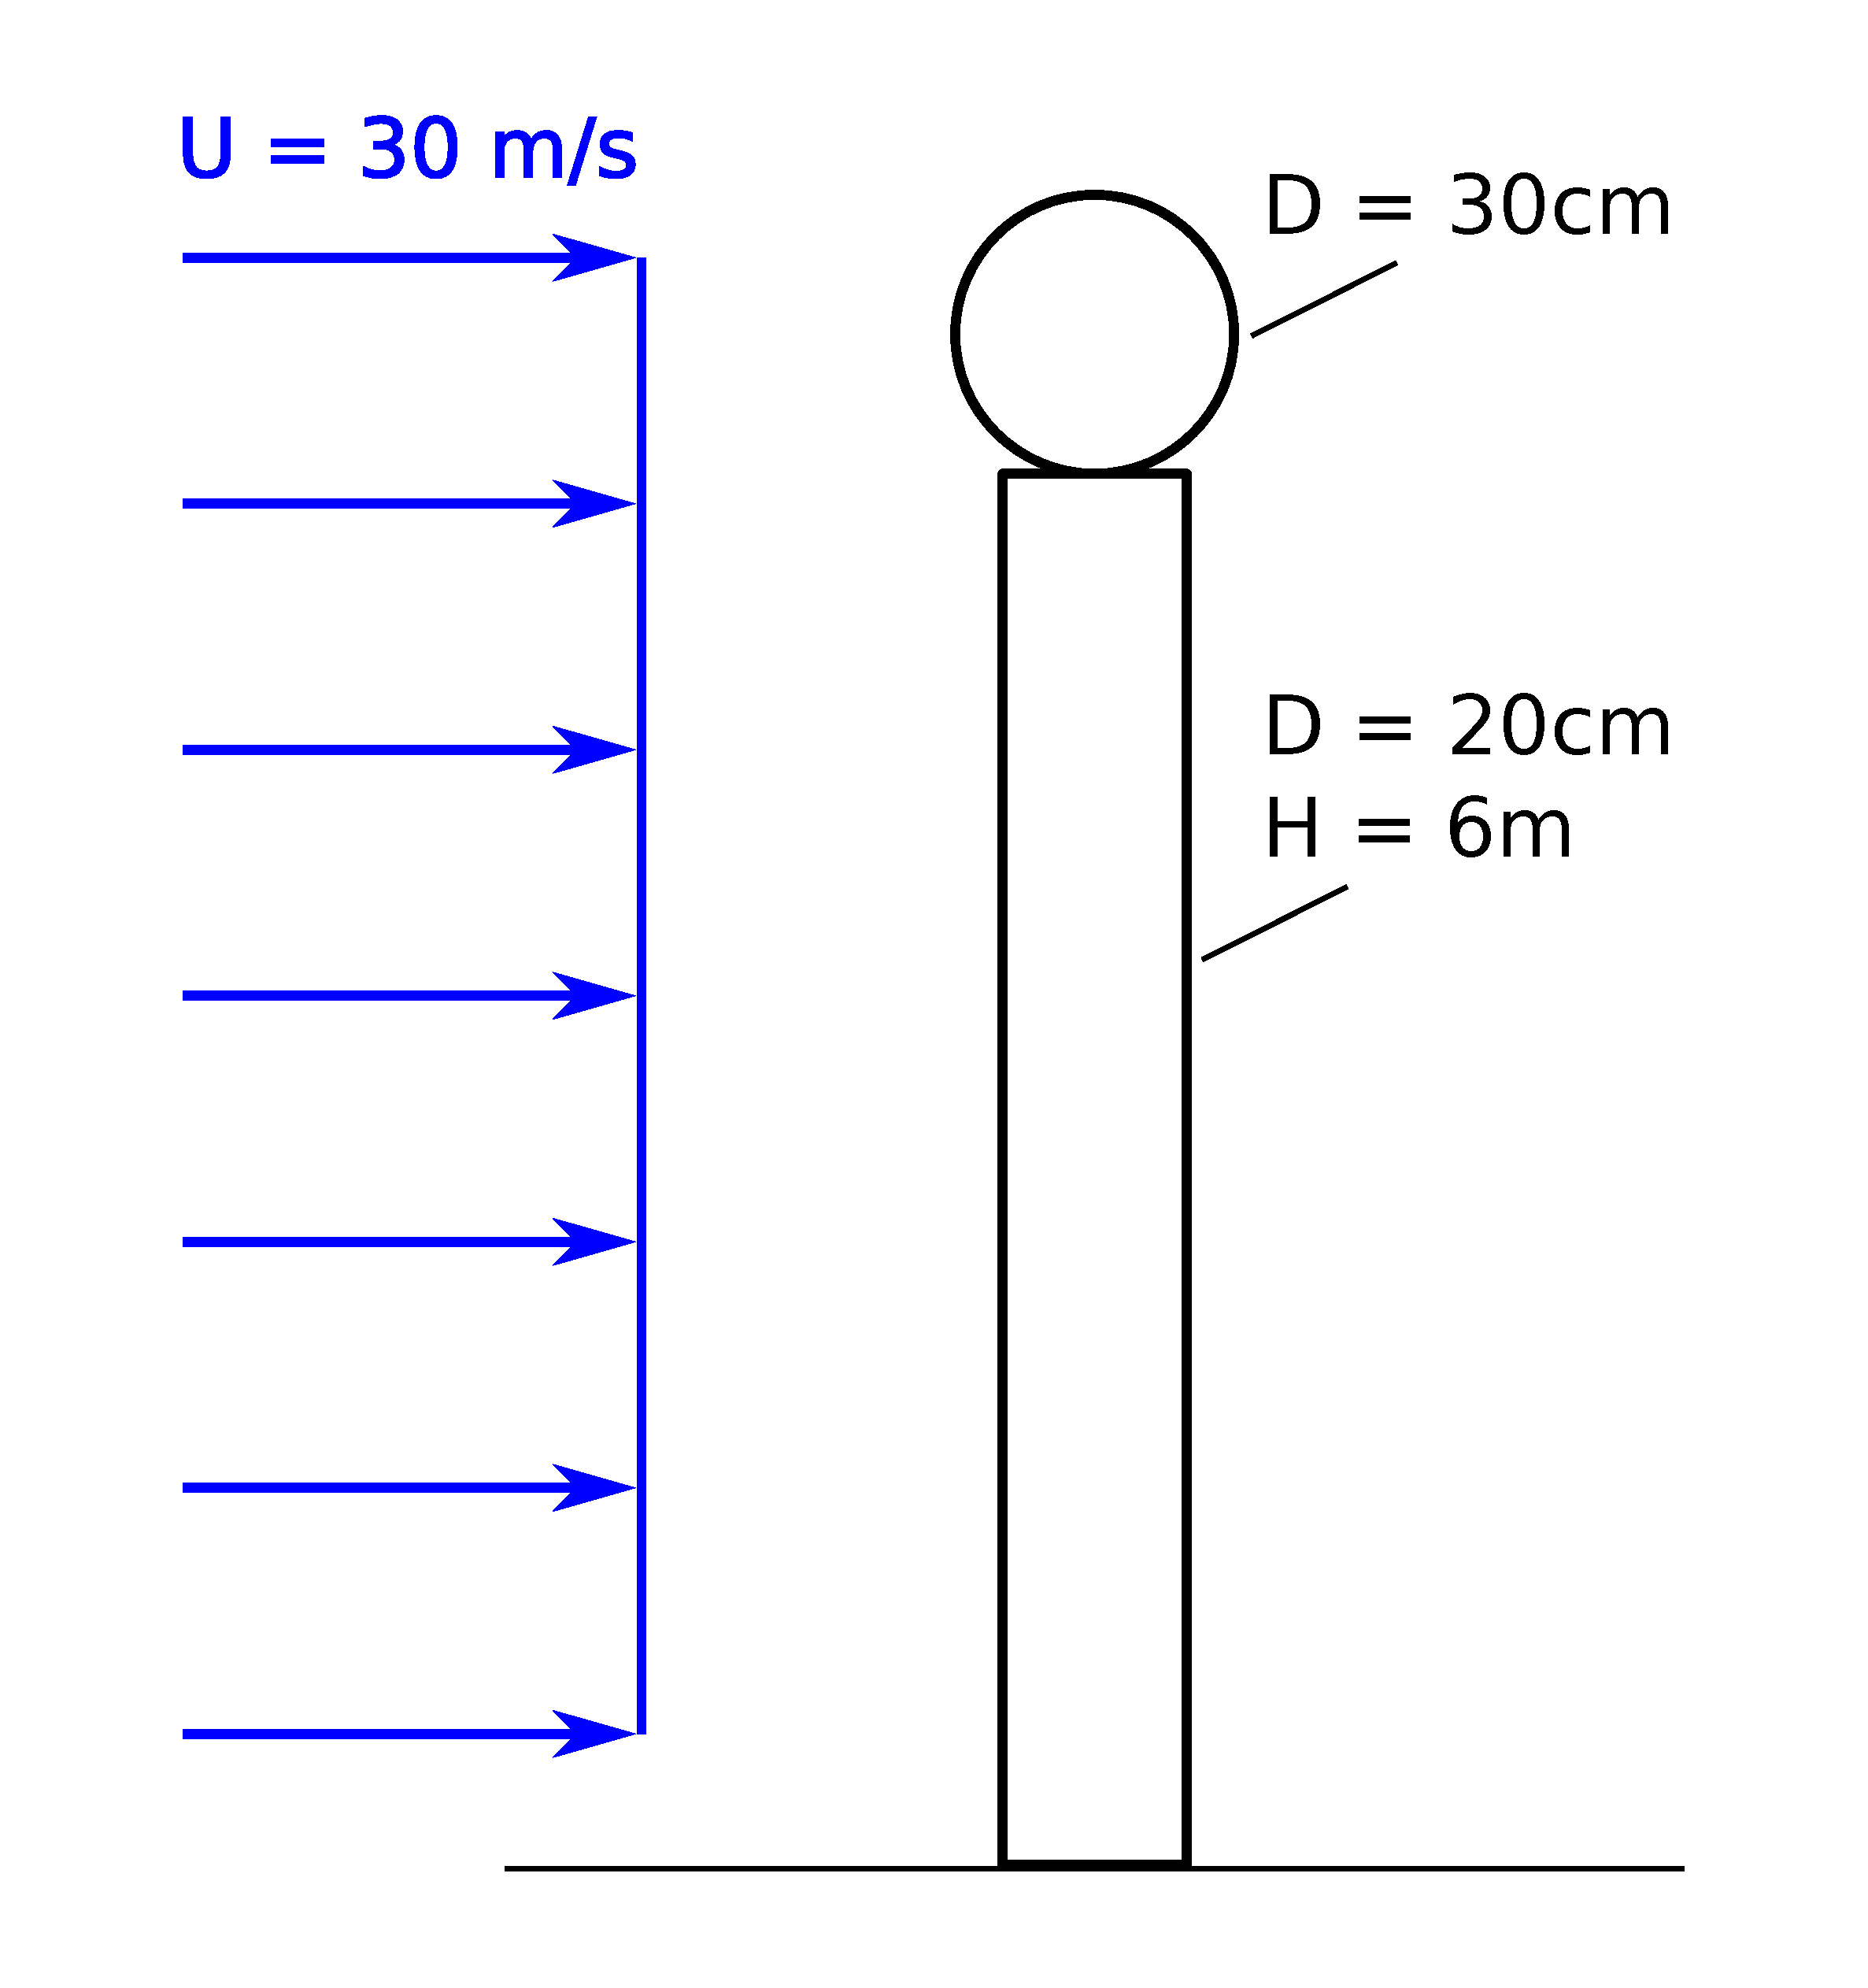
\includegraphics[width=0.35\textwidth]{Figures/poste.eps}
\caption{\label{fig:fig2} }
\end{figure}

\newpage

\underline {Problema 3:}
\vspace{0.2cm}

Una esfera cuyo di\'ametro es de $50$\,cm y $SG=1.05$, se deja caer en un estanque de agua a $20^\circ$C. Calcule la velocidad terminal de la esfera.
\vspace{0.2cm}

\underline {Problema 4 (P. 17.11M Mott\footnote{footnotes working fine}):}
\vspace{0.2cm}

Un tipo de indicador de nivel incorpora cuatro tasas hemisféricas con sus frentes abiertos montados, como se muestra en la figura~\ref{fig:fig3}. Cada tasa mide 15 mm de diámetro. Un motor las impulsa a velocidad de rotación constante. Calcule el torque que debe producir el motor para mantener el movimiento a 20 rev/min, cuando las tasas están en:
\begin{enumerate}
\item aire a 30 °C, y
\item gasolina a 20 °C.
\end{enumerate}

\begin{figure}[H]
\centering\includegraphics[width=0.4\textwidth]{Figures/17_11M.png}
\caption{\label{fig:fig3} }
\end{figure}

\footnotetext{Mott, Robert L. Mecanica de Fluidos 6/e. Pearson educación, 2006.}

%%%%%%%%%%%%%%%%%%%%%%%%%
%%%%%%%%%%%%%%%%%%%%%%%%%
%%%%%%%%%%%%%%%%%%%%%%%%%
\end{document}
